\documentclass[
  %fleqn,     das ist für die zentrierung
	parskip=half,
	captions=tableheading,
  titlepage=firstiscover, 		%************************************************** by Rk
	bibliography=totoc		%*************************************by Rk
	]{scrartcl}			
% \usepackage{etex}
% \reserveinserts{28}

%Das ist für die Kopfzeile
\usepackage[headsepline]{scrlayer-scrpage}
\pagestyle{scrheadings}
\clearpairofpagestyles
\ofoot{\pagemark}
\ohead{\headmark}
\automark{section}

% Warnung, falls nochmal kompiliert werden muss		%*************************************by Rk
\usepackage[aux]{rerunfilecheck}

% unverzichtbare Mathe-Befehle
\usepackage{amsmath}
% viele Mathe-Symbole
\usepackage{amssymb}
% Erweiterungen für amsmath
\usepackage{mathtools}
\usepackage{upgreek}
% Fonteinstellungen
\usepackage{fontspec}				%************************************************** by Rk
% Latin Modern Fonts werden automatisch geladen
% Latin Modern Fonts werden automatisch geladen
% Alternativ zum Beispiel:
%\setromanfont{Libertinus Serif}
%\setsansfont{Libertinus Sans}
%\setmonofont{Libertinus Mono}

\usepackage{polyglossia}
\usepackage[				%************************************************** by Rk
	backend=biber,
]{biblatex}  	
%Quellendatenbank	
\setmainlanguage{german}			
\addbibresource{lit.bib}		%************************************************** by Rk


\usepackage{expl3}
\usepackage{xparse}

\usepackage{physics}

\usepackage[unicode, german]{hyperref}
\usepackage[autostyle]{csquotes}
\usepackage[
  math-style=ISO,    % ┐
  bold-style=ISO,    % │
  sans-style=italic, % │ ISO-Standard folgen
  nabla=upright,     % │
  partial=upright,   % ┘
  warnings-off={           % ┐
    mathtools-colon,       % │ unnötige Warnungen ausschalten
    mathtools-overbracket, % │
  },                       % ┘
]{unicode-math}

% traditionelle Fonts für Mathematik
\setmathfont{Latin Modern Math}
% Alternativ zum Beispiel:
%\setmathfont{Libertinus Math}

\setmathfont{XITS Math}[range={scr, bfscr}]
\setmathfont{XITS Math}[range={cal, bfcal}, StylisticSet=1]

% Zahlen und Einheiten
\usepackage[
  locale=DE,                 % deutsche Einstellungen
  separate-uncertainty=true, % immer Fehler mit \pm
  per-mode=symbol-or-fraction,       % ^-1 für inverse Einheiten
  % output-decimal-marker=.,   % . statt , für Dezimalzahlen
]{siunitx}

% chemische Formeln
\usepackage[
  version=4,
  math-greek=default, % ┐ mit unicode-math zusammenarbeiten
  text-greek=default, % ┘
]{mhchem}

% Wenn man andere Schriftarten gesetzt hat,
% sollte man das Seiten-Layout neu berechnen lassen
\recalctypearea{}				%************************************************** by Rk


% richtige Anführungszeichen 
\usepackage[autostyle]{csquotes}

% schöne Brüche im Text
\usepackage{xfrac}

% Grafiken können eingebunden werden
\usepackage{graphicx}
% größere Variation von Dateinamen möglich
% \usepackage{grffile}
\usepackage{scrhack}

% Verbesserungen am Schriftbild
\usepackage{microtype}

% Standardplatzierung für Floats einstellen
\usepackage{float}
\usepackage[section, below]{placeins}
% \usepackage[..]{caption}
\floatplacement{figure}{htbp}
\floatplacement{table}{htbp}

\usepackage{booktabs}
\usepackage{subcaption}
% \usepackage{subfig}
\author{%
  Raphael Rico Kaiser\\%
  \href{raphael.kaiser@tu-dortmund.de}{raphael.kaiser@tu-dortmund.de}%
  \texorpdfstring{\and}{,}%
  Hendrik Trojan\\%
  \href{hendrik.trojan@tu-dortmund.de}{hendrik.trojan@tu-dortmund.de}%
}

\publishers{TU Dortmund - Fakultät Physik}
\usepackage{romannum}
\AtBeginDocument{\pagenumbering{arabic}}

\NewDocumentCommand \e {}
{
  \symup{e}
}

\NewDocumentCommand \const {}
{
  \text{const.}
}

\NewDocumentCommand \fig {mmm}
{
\begin{figure}
    \centering 
    \includegraphics[width=9cm]{#1}
    \caption{#3}
    \label{#2}
   \end{figure}
\nocite{*}
}

\usepackage{romannum}
\usepackage{listings}
\lstset{numbers=left, numberstyle=\tiny, numbersep=5pt}
\lstset{language=Perl}
\AtBeginDocument{\pagenumbering{arabic}}

\title{
\includegraphics[scale=0.8]{../logo.jpg} \\ \vspace*{1cm} V49 \\ - Gepulste NMR -}

%\title{test}
\date{Durchführung: 17.01.2021, Abgabe: 27.01.2021}

\begin{document}

\maketitle

\tableofcontents
\newpage

\section{Ziel}
In diesem Versuch sollen die Spin-Gitter- und die Spin-Spin-Relaxationszeit sowie der Diffusionskoeffizient von bidestilliertem Wasser mit Hilfe magnetischer Kernspinresonanz (NMR) bestimmt werden.


\section{Theorie}
\label{sec:Theorie}

\subsection{Magnetisierung} %?
Die in diesem Versuch genutzte magnetische Kernspinresonanz ist der Effekt, bei dem die magnetischen Momente der Atomkerne mit einem äußeren Magnetfeld bzw. einem internen elektromagnetischen Feld wechselwirken.
Die Kernspinresonanz basiert auf der Larmorpräzession der Kernspins um die Achse eines konstanten Magnetfelds (siehe \autoref{fig:larmor}).
Die Kernspins orientieren sich zum Magnetfeld, wenn die emittierten oder absorbierten magnetischen Wechselfelder mit der Larmorpräzession in Resonanz sind.

\begin{figure}
    \centering
    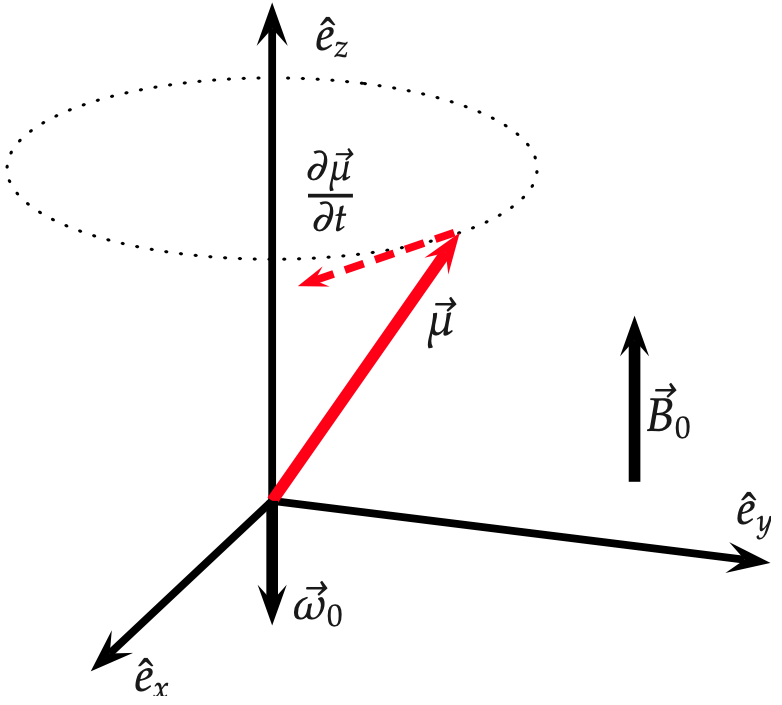
\includegraphics[width=0.3\linewidth]{./figures/larmor.png}
    \caption{Darstellung der Larmorpräzession eines Spins in einem statischen Magnetfeld $\vec{B}_0$ im Laborsystem. \cite{Anleitung}}
    \label{fig:larmor}
\end{figure}

Durch ein externes statisches Magnetfeld richten sich die magnetischen Momente der Kerne teilweise aus und es entsteht eine makroskopische Magnetisierung $\vec{M}$. Diese beschreibt die Summe aller Einzelmomente pro Volumeneinheit. %
Bei Spin $\frac{1}{2}$ Teilchen (z.B. Protonen) liegt in einem Magnetfeld eine Aufspaltung in zwei Unterniveaus mit Quantenzahlen $m= \pm \frac{1}{2}$ vor. % oder?
%noch mehr???



\subsection{Relaxationseffekte}
Durch Einstrahlung von Hochfrequenzquanten wird die Magnetisierung aus dem thermischen Gleichgewicht gebracht.
%Sagen was Relaxation ist?
Der Verlauf der Relaxation kann durch die Bloch-Gleichungen beschrieben werden. %bzw Zeitentwicklung der Magnetisierung
Im rotierenden Koordinatensystem lauten diese wie folgt %und ohne RW Feld im Resonanzfall ?
\begin{align}
    \left( \frac{d M_x}{dt} \right)_{RKS} &= \left( - \frac{M_x}{T_2} \right) \\
    \left( \frac{d M_y}{dt} \right)_{RKS} &= \left( - \frac{M_y}{T_2} \right) \\
    \left( \frac{d M_z}{dt} \right)_{RKS} &= \left( - \frac{M_z - M_{\infty}}{T_2} \right) \, .
    \label{eq:bloch}
\end{align} 
Es werden zwei Arten von Relaxationseffekten unterschieden, welche im Folgenden kurz beschrieben werden.

\textbf{Spin-Gitter-Relaxation} \newline
Ohne Magnetfeld sind die Spinniveaus gleichbesetzt und es gibt keine makroskopische Magnetisierung. Nach Anlegen eines Magnetfelds orientiert sich ein Überschuss der Kernmomente in Magnetfeldrichtung und im Limes ist die Magnetisierung im thermischen Gleichgewicht $\vec{M}_{\infty} || \vec{e}_z$, welches als unendlich hohe Temperatur des Spinsystems beschrieben werden kann.
Das Spinsystem beginnt sich abzukühlen und die Besetzungszahlen stellen sich auf das thermische Gleichgewicht ein. Dabei geben die Kerne Energie an das Gitter ab.
%Der Vorgang wird auch longitudinale Relaxation genannt.
Die Spin-Gitter- oder longitudinale Relaxationszeit ($T_1$) gibt die Dauer an, bis die Energie des Spinsystems in Gitterschwingungen übergeht.

\textbf{Spin-Spin-Relaxation} \newline
Die Magnetisierung wird mittels eines Pulses in die x-y-Ebene gekippt. Diese präzediert dann um das Magnetfeld. Durch die Spin-Gitter-Relaxation wird die Magnetisierung wieder in z-Richtung gekippt. Die Phasenbeziehung der Kernspins geht durch fluktuierende Felder verloren (Dephasierung), weshalb die erzeugte Quermagnetisierung zerfällt.
Die Spin-Spin- oder transversale Relaxationszeit ($T_2$) gibt die Dauer dieses Zerfalls an.

\subsection{Einstrahlung von HF-Pulsen}
In diesem Versuch werden resonante Hochfrequenzpulse eingestrahlt, um die Zeitentwicklung der Magnetisierung zu beobachten.
Das bedeutet, dass ein Feld $\vec{B}_1$ für die Zeit $t_p$ eingeschaltet wird. Dieses wird durch eine senkrecht zu dem statischen Feld $\vec{B}_0$ orientierte Spule induziert.
Der Drehwinkel der Magnetisierung um die $x_{RKS}$- bzw. $y_{RKS}$- Achse ist durch
\begin{equation*}
    \alpha = | \omega_1 | \, t_p = \gamma B_1 t_p
\end{equation*}
gegeben, wobei $\gamma$ das gyromagnetische Verhältnis ist.
In diesem Versuch werden Pulslängen benötigt, die die Magnetisierung um $90 \degree$ und um $180 \degree$ drehen. Eine $90 \degree$-Drehung wird mit einer Pulslänge von 
\begin{equation*}
    \Delta t_{90} = \frac{\pi}{2 \gamma B_1}
\end{equation*}
erreicht. Für eine $180 \degree$-Drehung ist die doppelte Pulslänge erforderlich.


\subsection{Diffusionsverhalten einer Flüssigkeit}
Die Kernspins einer Flüssigkeit diffundieren und unterliegen wegen des inhomogenen Magnetfelds unterschiedlichen Feldstärken. Die Magnetisierungsamplitude der Spin-Echos nimmt exponentiell mit der Zeitkonstante
\begin{equation*}
    T_D = \frac{3}{2 D \gamma^2 g^2}
\end{equation*}
ab und ist durch
\begin{equation*}
    M(\tau) = M_0 \exp(- \frac{2 \tau}{T_2}) \exp(- \frac{\tau^3}{T_D}) %in der langen Anleitung steht M(2 \tau) ?
\end{equation*}
beschrieben, wobei $D$ die Diffusionskonstante und $g$ der Gradient des Magnetfeldes ist.

Mit Hilfe der Stokeschen Formel
\begin{equation*}
    D = \frac{k_B T}{6 \pi \eta r}
\end{equation*}
kann aus der Diffusionskonstanten der Molekülradius der Probenmoleküle bestimmt werden. Dabei ist $\eta$ die Viskosität der Probe.


\section{Messverfahren und Aufbau}

%Das Prinzip der verwendeten Apparatur ist in \autoref{fig:aufbau} zu sehen.
Der Versuchsaufbau besteht prinzipiell aus einem Permanentmagneten, der ein homogenes Magnetfeld $B_0 \vec{e}_z$ erzeugt. Die Probe befindet sich in einer Spule, welche sowohl mit einem Sender als auch einem Empfänger gekoppelt ist. Es können also hochfrequente Pulse erzeugt und die entstandene Magnetisierung gemessen werden. %
%\begin{figure}
%    \centering
%    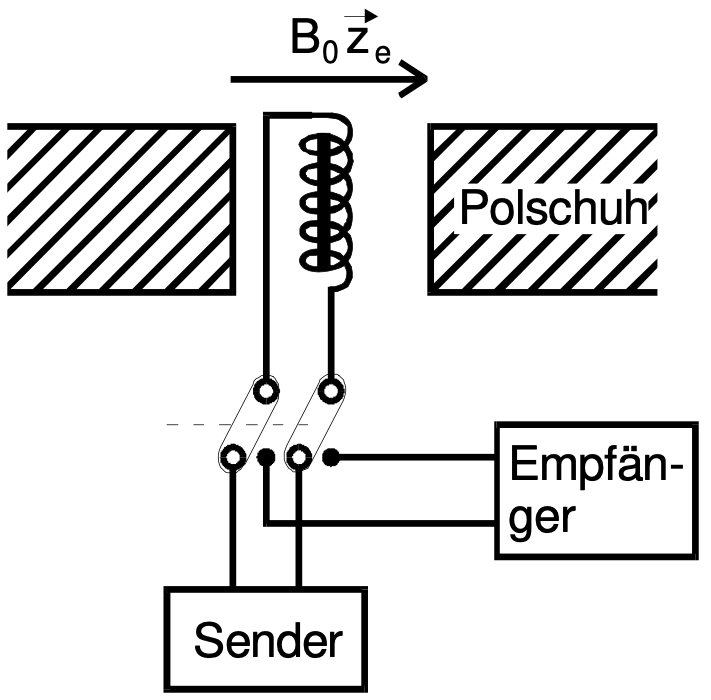
\includegraphics[width=0.4\linewidth]{./figures/aufbau.png}
%    \caption{Der Aufbau. \cite{Anleitung}}
%    \label{fig:aufbau}
%\end{figure}



%\subsection{Quadraturdetektion} %entfernen?

%Das Signal der FID kann mit zwei Referenzsignalen mit $\omega_{Ref}$, die um 90° zueinander phasenverschoben sind, gemischt werden. Dieses Mischen in Kombination mit einem Tiefpassfilter führt dazu, dass die resultierenden Spannungen $U_1$ und $U_2$ genau den Magnetisierungen $(M_x)_{RKS}$ und $(M_y)_{RKW}$ entsprechen, wenn $\omega_{Ref} - \omega_0 = 0$ und die richtige Phasenlage gefunden wurde.



\subsection{Methode zur Messung der Spin-Gitter-Relaxationszeit}
Diese Methode wird "inversion recovery" genannt.
Die Magnetisierung wird mittels eines $180 \degree$ Pulses in negative z-Richtung gekippt. Nach der Zeit $\tau$ wird ein $90 \degree$ Puls gesendet, welcher den z-Anteil in die x-y-Ebene dreht. %und die Amplitude wird gemessen.
Mit den Anfangsbedingungen $M_x(0) = M_y(0) = 0$ und $M_z(0) = - M_0$ gilt für die Amplitude 
\begin{equation*}
    M(\tau) = M_0 \left( 1 - 2 \exp(- \frac{\tau}{T_1}) \right) \, .
\end{equation*}
Dies folgt aus den Bloch'schen Gleichungen (\autoref{eq:bloch}). Die Spin-Gitter-Relaxationszeit $T_1$ kann durch Variation der Dauer $\tau$ zwischen den Pulsen bestimmt werden.

\begin{figure}
    \centering
    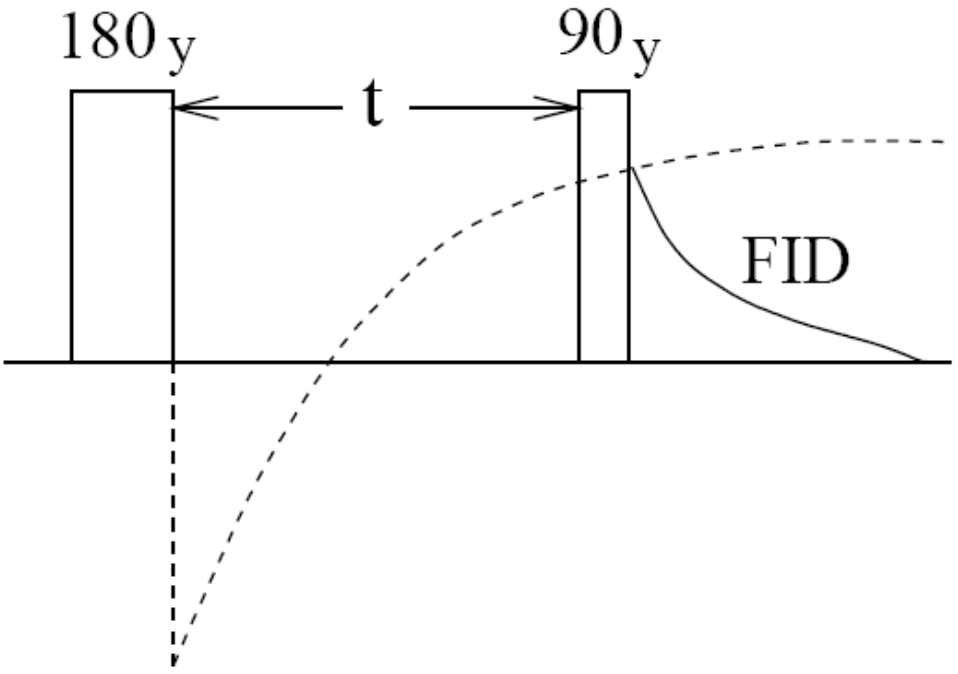
\includegraphics[width=0.5\linewidth]{./figures/inversion_recovery.png}
    \caption{Inversion Recovery Methode zur Bestimmung der Spin-Gitter-Relaxationszeit. \cite{Anleitung}}
    \label{fig:inv_rec}
\end{figure}



\subsection{Methoden zur Messung der Spin-Spin-Relaxationszeit}

Bei einem $90 \degree$ Puls wird die Magnetisierung in die x-y-Ebene gekippt und relaxiert zurück in das thermische Gleichgewicht. Aufgrund des sich ändernden Magnetfelds wird ein Induktionsstrom erzeugt. Die Amplitude nimmt wegen der Spin-Spin-Relaxation ab und zerfällt mit $T_2$. Das wird freier Induktionszerfall (FID) genannt.

Für ein homogenes Magnetfeld ist der Zerfall des FID durch die Spin-Spin-Relaxation gegeben.
Da das statische Magnetfeld in der Realität Inhomogenitäten aufweist, kann nur die effektive Abfall-Zeit bestimmt werden. Diese kann durch
\begin{equation*}
    \frac{1}{T^{eff}_2} = \frac{1}{T_2} + \frac{1}{T^{inhom}_2}
\end{equation*}
beschrieben werden und ist in der Regel kürzer als $T_2$.
Dieser Effekt kann wie im Folgenden beschrieben durch bestimmte Pulsfolgen eliminiert werden. %\autoref{sec:spinecho}.


\subsubsection{Spin-Echo-Methode}
\label{sec:spinecho}
Bei dem Spin-Echo-Verfahren werden zwei Pulse eingespeist. Der erste Puls ist ein $90 \degree$- Puls.
Am Ende des FID zur Zeit $\tau$, wenn alle Spins dephasiert sind und daher kein Signal mehr messbar ist, wird ein $180 \degree$-Puls auf die Probe gegeben. Als Resultat laufen die dephasierenden Spins zum Zeitpunkt $2\tau$ wieder zusammen und es entsteht ein Signal mit umgekehrtem Vorzeichen und niedrigerer Amplitude
\begin{equation*}
    M(2\tau) = M(0) \exp(-\frac{2\tau}{T_2}) \, .
\end{equation*}
Aus der exponentiellen Abnahme der Amplituden lässt sich so die Relaxationszeit bestimmen.
%noch was zur Diffusion?

\begin{figure}
    \centering
    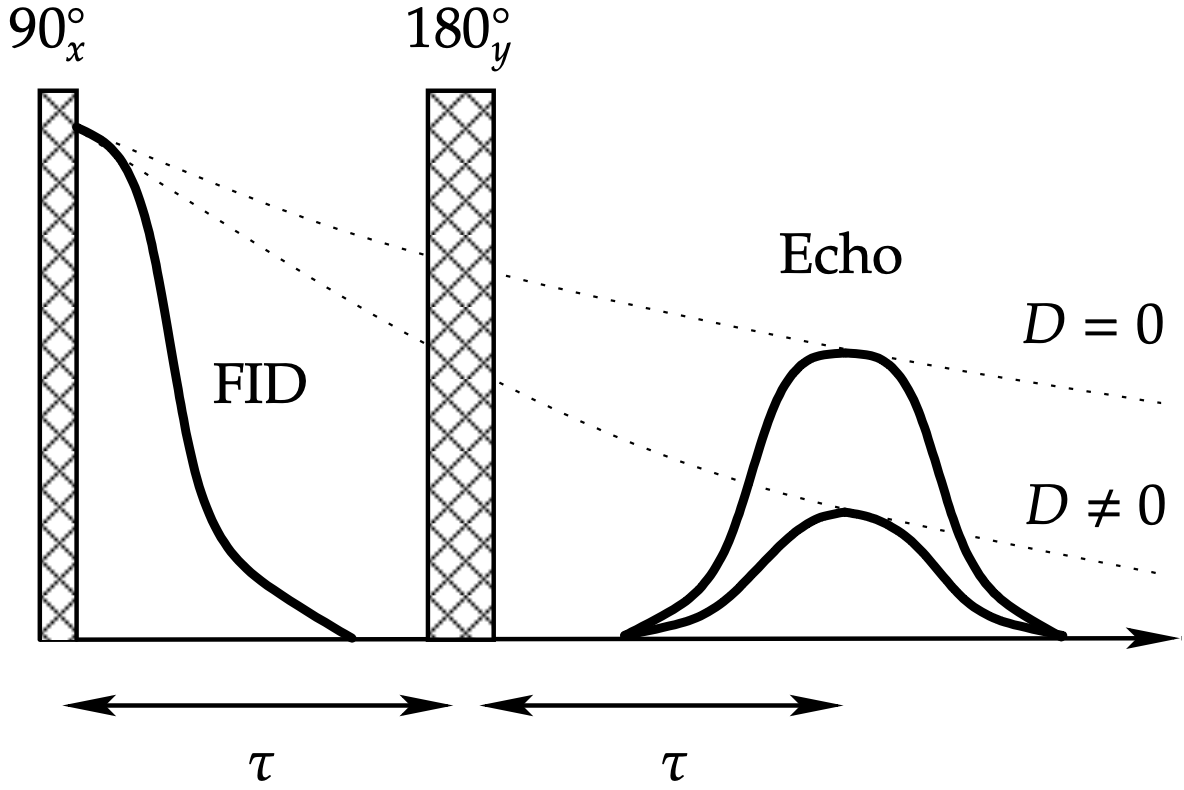
\includegraphics[width=0.5\linewidth]{./figures/spinecho.png}
    \caption{Spin-Echo-Methode zur Bestimmung der Spin-Spin-Relaxationszeit. Zu sehen ist auch der Einfluss der Diffusion auf das Echo. \cite{Anleitung}}
    \label{fig:spinecho}
\end{figure}

\subsubsection{Carr-Purcell-Methode}
Bei der Carr-Purcell-Methode können mehrere Spinechos hintereinander beobachtet werden, indem weitere $180 \degree$-Pulse jeweils im Abstand von $2 \tau$ verwendet werden. Auf diese Weise wird die lange Wartezeit zwischen den Messungen, welche bei der Spin-Echo-Methode nötig ist, damit sich die Gleichgewichtslage wieder einstellen kann, verkürzt.
Problematisch bei dieser Methode ist, dass durch Justagefehler bei der Dauer der $180 \degree$-Pulse die Magnetisierung mit steigender Zahl der Pulse immer weiter von der x-y-Ebene abweicht.

%Nachteilig an der Spin-Echo-Methode ist die lange Wartezeit, da mit einer neuen Messung gewartet werden muss, bis sich die Gleichgewichtslage wieder eingestellt hat. Hier bietet es sich an, gleich mehrere 180-Grad-Pulse in gleichen Abständen $2\tau$ auf die Probe zu geben, sodass eine ganze Reihe von Spin-Echos aufgenommen werden kann. 


\subsubsection{Meiboom-Gill-Methode}
Die Verstärkung der Fehler bei der Carr-Purcell-Methode kann durch die Meiboom-Gill-Methode ausgeglichen werden. Durch eine spezielle Vorrichtung wird die Phase der $180 \degree$-Pulse um $90 \degree$ gegenüber dem $90 \degree$-Puls gedreht. 
Für geradzahlige Echos kompensieren sich die Fehler und die Amplituden haben den richtigen Wert. %?



\section{Durchführung}
\label{sec:Durchführung}

\subsection{Justage und Temperaturmessung}
In den Aufbau wird zunächst eine Kalibrationsprobe aus Wasser mit Kupfersulfat eingebracht. Das Kupfersulfat verkürzt die Relaxationszeit und wird nur für eine schnellere Justage benutzt.
Es werden die Startparameter eingestellt, welche in \autoref{tab:params} aufgelistet sind. Die Parameter werden nun iterativ eingestellt. %Die finalen Werte sind ebenfalls in \autoref{tab:params} zu sehen.

Die Frequenz des Referenzsignals wird so eingestellt, dass die FID Messung keine Oszillationen enthält. 
Durch Einstellen der Phase wird die Amplitude eines Signals zum Zeitpunkt $t=0$ auf Null, bzw. auf ihren minimalen Wert, verschoben. 
%Diese ist hauptsächlich auf einem der Kanäle zu sehen, welcher als Realteil angenommen wird. %oder???
Die Feldhomogenität wird maximiert (engl. shimmen), indem der Gradient so eingestellt wird, dass die Abklingzeit des FID möglichst lang ist. Das ist durch Einstellen der Shims x, y, z und $z^2$ möglich.
Die Pulslängen für die $90 \degree$- und $180 \degree$-Pulse 
werden so eingestellt, dass die Amplitude des FID bei $90 \degree$ maximal und bei $180 \degree$ minimal ist. %

Die Temperatur in der Spule wird mit einem Thermoelement gemessen.
Die Temperaturmessung wird nach den Messungen in \autoref{sec:T2Messung} und \autoref{sec:Diffusionsmessung} wiederholt.

Nach der Justage wird die Kalibrationsprobe durch bidestilliertes (also hochreines) Wasser ersetzt.

\begin{table}
  \centering
  \caption{Die Startwerte der Parameter.}
  \label{tab:params}
  \begin{tabular}{l l}
    \toprule
    Parameter & Startwert \\
    \midrule
    Frequenz & $f = \SI{21.7}{\mega\hertz}$ \\
    Pulslänge & $A = \SI{2}{\micro\second}$ \\
    Anzahl der B-Pulse & $N = \num{0}$ \\
    Periode & $P = \SI{0.5}{\second}$ \\
    Shims & $x=\num{-1.0}$ \\
      & $y=\num{-5.0}$ \\
      & $z=\num{3.7}$ \\
      & $z^2=\num{-2.4}$ \\
    \bottomrule
  \end{tabular}
\end{table}

\subsection{Messung der Spin-Gitter-Relaxationszeit}
Die Pulslänge A wird so eingestellt, dass ein $180 \degree$-Puls gesendet wird und Pulslänge B wird so eingestellt, dass ein $90 \degree$-Puls gesendet wird. %Formulierung
Die Anzahl der B-Pulse beträgt $N=1$.
Anschließend wird der Pulsabstand $\tau$ variiert und die FID Amplitude abgelesen. 
%Dabei liegen die Messpunkte äquidistant auf einer logarithmischen Achse.

\subsection{Messung der Spin-Spin-Relaxationszeit}
\label{sec:T2Messung}
Für diese Messung wird die A Pulslänge auf $90 \degree$ und die B Pulslänge auf $180 \degree$ eingestellt.
Die Anzahl der B-Pulse beträgt $N=100$.
Der "MG"-Schalter wird auf "on" gestellt. Es wird ein Bild aller Peaks mit dem Oszilloskop gespeichert. Der Schalter wird auf "off" gestellt und es wird ein Vergleichsbild gespeichert. Es werden also die Signalverläufe für eine Messung mit und ohne Meiboom-Gill-Methode gespeichert.


\subsection{Messung der Diffusion}
\label{sec:Diffusionsmessung}
Für die Diffusionsmessung wird der z-Gradient maximiert. Die Anzahl der B-Pulse wird wieder auf $N=1$ gestellt. Der Pulsabstand wird variiert und die Höhe des Echos abgelesen. Für ein gut sichtbares Echo wird das Signal von beiden Kanälen gespeichert.


%\subsection{Messung der Viskosität}
%Damit der Molekülradius aus der Diffusionskonstante bestimmt werden kann, muss zunächst die Viskosität bestimmt werden. Diese wird mit Hilfe eines Viskosimeters gemessen, indem die Zeit gestoppt wird, die das Wasser zum Zurücklegen der Strecke zwischen zwei Markierungen braucht.


\newpage
\section{Auswertung}
Im folgenden Abschnitt werden die gesammelten Messdaten ausgewertet und analysiert.
\subsection{Justage}
Bevor mit den eigentlichen Messungen begonnen werden kann, müssen einige Justierungen vorgenommen werden.
Die Shim-Parameter sind in \autoref{tab:shim} dargestellt und gelten für die Bestimmung
von $T_1$ und $T_2$.
\begin{table}
  \centering
  \caption{Verwendete Shim-Parameter.}
  \label{tab:shim}
  \begin{tabular}{c c c c}
    \toprule
    x & y & z & $\symup{z^2}$ \\
    \midrule
    -1.0 & -4.2 & +4.1 & -2.24 \\
    \bottomrule
  \end{tabular}
\end{table}
\FloatBarrier
Der Imaginärteil der Schwingung verschwindet für eine eingestellte Phase von $\phi=-64°$.
Für eine Frequenz von $f=\SI{21,719 }{\mega\hertz}$ weisen beide Signale Real- und Imaginärteil
keine Oszillationen mehr auf.


\subsection{Bestimmung der Spin-Gitter-Relaxationszeit T1}
Für die Messung der Spin-Gitter Relaxationszeit $T_1$ wird die $90°$
Pulslänge ($\tau_\text{90}$) auf $\SI{2,5}{\micro\second}$ und die $180°$ Pulslänge ($\tau_\text{180}$) auf
$\SI{5,08}{\micro\second}$ gestellt.
Die Messwerte sind in \autoref{tab:t1}  und der Plot in \autoref{fig:T1} zu finden.
Mit Hilfe der Funktion
\begin{equation*}
  M\left(\tau\right) = M_0 \left(1-2\exp(-\frac{\tau}{T_1})\right)
\end{equation*}
findet eine Ausgleichsrechnung statt.
Der Fit liefert die Fitparameter 
\begin{align*}
    M_0 &= \SI{1086 \pm 7}{\mV}\\% \label{eqn:M0_T1} \\
    T_1 &= \SI{2,565 \pm 0,034 }{\second}.% \label{eqn:T1}.
\end{align*}
\input{build/tabT1.tex}
\begin{figure}
    \centering
    \includegraphics[width=0.7\linewidth]{build/T1.pdf}
    \caption{Plot für die Bestimmung der Spin-Gitter Relaxationszeit.}
    \label{fig:T1}
\end{figure}
\FloatBarrier
\subsection{Bestimmung der Spin-Spin-Relaxationszeit T2}
\subsubsection{Die Meiboom-Gill-Methode}
In diesem Versuchsteil wird mittels der Meiboom-Gill-Methode 
die Spin-Gitter-Relaxationszeit $T_2$ bestimmt.
Der Graph welcher mit der Meiboom-Gill-Methode entstanden ist, ist in \autoref{fig:mei}
zu sehen.
\begin{figure}
  \centering
  \includegraphics[width=0.7\linewidth]{build/MG.pdf}
  \caption{Signalverlauf unter der Anwendung der Meiboom-Gill-Methode.}
  \label{fig:mei}
\end{figure}
Um im nächsten Schritt die Relaxationszeit $T_2$ zu bestimmen, werden die 
einzelnen Peaks in \autoref{fig:mei} in einen neuen Graphen in Abhängigkeit der Zeit aufgetragen.
Dieser Graph ist in \autoref{fig:mei_fit} zu sehen.
Mit Hilfe der Funktion
\begin{equation*}
  M\left(t\right) = M_0 \exp(-\frac{t}{T_2})
\end{equation*} 
wird der Graph gefittet.
Der Fit liefert die Fitparameter 
\begin{align*}
    M_0 &= \SI{1025 \pm 5}{\mV}\\ % \label{eqn:M0_T2} \\
    T_2 &= \SI{1,696 \pm 0,019 }{\second}.% \label{eqn:T2}.
\end{align*}
\begin{figure}
  \centering
  \includegraphics[width=0.7\linewidth]{build/peaks.pdf}
  \caption{Darstellung der einzelnen Peak der Meiboom-Gill-Methode.}
  \label{fig:mei_fit}
\end{figure}
\FloatBarrier
\subsubsection{Die Carr-Purcell-Methode}
Eine andere Methode um die Relaxationszeit $T_2$ zu bestimmen ist die Carr-Purcell-Methode.
Allerdings muss bei dieser darauf geachtet werden, dass die Pulslänge des 180° Pulses exakt
eingestellt wird.
Dies ist aber experimentell in unserem Versuch nicht realisierbar und würde zu großen
Abweichungen führen.
In \autoref{fig:carr} ist der Vollständigkeit halber der Graph der Carr-Purcell-Methode abgebildet.
\begin{figure}
    \centering
    \includegraphics[width=0.7\linewidth]{build/carr_purcell.pdf}
    \caption{Graph der Carr-Purcell-Methode.}
    \label{fig:carr}
\end{figure} 

\subsection{Bestimmung der Diffusionskonstanten}
Um die Diffusionskonstante der Probe zu bestimmen, wird als erster Schritt die Diffusionszeit
$T_D$ ermittelt.
Die aufgenommenen Messwerte sind in \autoref{tab:echo_2} dargestellt.
\input{build/tabEcho_2.tex}
Um die Diffusionszeit zu bestimmen, werden die gemessenen Echohöhen $M(\tau)$ in Abhängigkeit der Pulslänge $\tau$ in \autoref{fig:echo_2}
graphisch dargestellt.
\begin{figure}
  \centering
  \includegraphics[width=0.7\linewidth]{build/echo_2.pdf}
  \caption{Gemessene Echohöhen in Abhängigkeit der Pulslänge.}
  \label{fig:echo_2}
\end{figure}
Anschließend werden die Messdaten mit 
\begin{equation*}
  M\left(\tau\right) = M_0 \exp(-\frac{2\tau}{T_2}) \exp(-\frac{\tau^3}{T_D}) + M_1
\end{equation*}
gefittet.
Der Fit liefert die Fitparameter 
\begin{align*}
    M_0 &= \SI{1045 \pm 12}{\mV}\\% \label{eqn:M0_diff} \\
    M_1 &= \SI{41 \pm 12}{\mV}\\% \label{eqn:M1_diff} \\
    T_D &= \SI{1,40(5)e3}{\milli\second^3}.% \label{eqn:diff_zeit}.
\end{align*}
\FloatBarrier
\begin{figure}
  \centering
  \includegraphics[width=0.7\linewidth]{build/echo_gradient.pdf}
  \caption{Fouriertransformation des vollständigen Echos.}
  \label{fig:Fouriertransformation}
\end{figure}
\FloatBarrier
Nachdem die Diffusionszeit $T_D$ bestimmt worden ist,
wird im nächsten Schritt der Magnetfeldgradient mit Hilfe einer Fouriertransformation 
des vollständigen Echoverlaufs abgeschätzt.
Die Fouriertransformation ist in \autoref{fig:Fouriertransformation} zu sehen.
Aus der Fouriertransformation ergibt sich ein Durchmesser des halbkreisförmigen Verlaufes
$d_f \approx \SI{19,5}{\kilo\hertz}$.
Daraus folgt mit 
\begin{equation*}
  g = \frac{2 \pi d_f}{\gamma d}
\end{equation*}
ein Magnetfeldgradient $g=\SI{0,103}{\tesla \meter^{-1}}$. 
Hierbei ist $\gamma= \SI{267,5e6}{\second^{-1}\tesla^{-1}}$\cite{gyro_wiki} das 
gyromagnetische Verhältnis für Protonen und $d=\SI{4,2}{\milli\meter}$ der Probeninnendurchmesser.
Im letzten Schritt kann die Diffusionskonstante mit
\begin{equation*}
  D = \frac{3}{2 T_D \gamma^2 g^2} 
\end{equation*}
ermittelt werden.
Die Diffusionskonstante beträgt $D= \SI{1,40(5)e-9}{\meter^2\per\second}$.

\subsection{Bestimmung des Molekülradius}
Der Molekülradius kann mit Hilfe der Stokes-Formel berechnet werden.
Es gilt 
\begin{equation}
  r=\frac{k_\text{B}T}{6 \pi\eta D}.
  \label{eqn:r}
\end{equation}
Hierbei ist $T = \SI{294.75}{\kelvin}$ die gemessene Temperatur  
und $\eta = \SI{890.2}{\micro\pascal\second}$\cite{vis} die Viskosität.
Mit \autoref{eqn:r} ergibt sich ein Molekülradius von 
\begin{equation*}
  r = \SI{1.73(6)e-10}{\meter}.
\end{equation*}

Um einen Vergleichswert zu generieren, wird angenommen, dass die Moleküle 
in Wasser in der hexagonal dichtesten Kugelpackung angeordnet sind.
Die Einheitszelle besitzt in dieser Konstellation eine Füllung von ca. 74\%.
Die Dichte von Wasser bei einer Temperatur von $T = \SI{298.15}{\kelvin}$ ist 
$\rho=\SI{995}{\kilo\gram\per\metre^3}$\cite{dichte}. 
Das Molekülgewicht von Wasser beträgt $m = \frac{M_\text{mol}}{N_\text{A}} = \SI{2.99e-26}{\kilo\gram}$\cite{wasser}
Mit der Formel
\begin{equation*}
  r_\text{hcp} = \left(\frac{0,74 \, m}{\frac{4}{3}\pi\rho}\right)^{\frac{1}{3}}
\end{equation*}
ergibt sich ein Molekülradius von $r = \SI{1.74e-10}{\meter}$.
Die Abweichung vom Theoriewert beträgt somit ca. 1\%.


\section{Diskussion}
Zu Beginn der Diskussion kann gesagt werden, dass die Änderung der Temperatur während 
des gesamten Versuches eine wesentliche Fehlerquelle ist. 
Die Änderung der Temperatur ist zum einen durch das wiederholte Lüften des Raumes zustande gekommen und zum anderen 
durch den Erwärmungsvorgang des verwendeten Magneten.
Desweiteren kann nicht genau gesagt werden, ob das permanente Magnetfeld durch 
die unterschiedlichen Shim-Parameter in der Probe optimal homogenisiert worden ist.\\
Die gemessenen Relaxationszeiten sind 
\begin{align*}
  T_1 &= \SI{2,565 \pm 0,034 }{\second}\\
  T_2 &= \SI{1,696 \pm 0,019 }{\second}.
\end{align*}
Klar erkennbar ist, dass $T_1 > T_2$ ist, welches mit der Theorie übereinstimmt.
Werden die errechneten Werte direkt mit den Theoriewerten verglichen\cite{diff}
\begin{align*}
  T_\text{1,lit} &= \SI{3.09(15)}{\second},\\
  T_\text{2,lit} &= \SI{1.52(9)}{\second},
\end{align*}
ergibt sich für $T_1$ eine Abweichung von 16,99\% und für $T_2$ eine Abweichung von 10,37\%.

Die Diffusionskonstante hat in unserem Experiment den Wert 
\begin{equation*}
  D= \SI{1,40(5)e-9}{\meter^2\per\second}.
\end{equation*}
Verglichen mit dem Theoriewert\cite{diff} von 
\begin{equation*}
  D_\text{lit} = \SI{2.78(4)e-9}{\metre^2\per\second}
\end{equation*}
ergibt sich eine Abweichung von 49,64\%.
%Die Abweichung  warum so groß ? wegen halbkreisförmigen duch geschätzt,??

Der ermittle Molekülradius ist
\begin{equation*}
  r = \SI{1.73(6)e-10}{\meter}.
\end{equation*}
Verglichen mit dem Theoriewert von
\begin{equation*}
  r_\text{hcp}= \SI{1.74e-10}{\metre}
\end{equation*}
ergibt sich wie bereits erwähnt eine Abweichung von ca. 1\%.
Der ermittelte Wert scheint also sehr gut zu passen. 
Allerdings muss gesagt werden, dass für die Berechnung des Theoriewerts die Dichte von Wasser bei einer 
Temperatur von $\SI{25}{\celsius}$ verwendeten worden ist.
Im Experiment herrschte aber zu diesem Zeitpunkt eine Temperatur von nur $\SI{21,6}{\celsius}$.
Außerdem ist zur Berechnung die hexagonal dichteste Kugelpackung angenommen worden, 
welche den kleinsten Molekülradius liefert.
%\FloatBarrier
%\begin{figure}
%    \centering
%    \includegraphics[width=0.7\linewidth]{./figures/xxx.xxx}
%    \caption{xxx}
%    \label{fig:xxx}
%\end{figure}
%
%\begin{equation}\label{eq:xxx}    
%    \begin{split}
%        \lambda &= \SI{855}{\angstrom}\\
%        \delta_\text{ps} &= 0,6\cdot 10^{-6}\\
%        \delta_\text{si}&= 6,8\cdot 10^{-6} \\
%        n_\text{luft} &= 1 \\
%        n_\text{ps} &= 1 - \delta_\text{ps} \\
%        n_\text{si} &= 1 - \delta_\text{ps} 
%    \end{split}
%\end{equation}
\newpage
\nocite{*}
\printbibliography{}
\end{document}